$  $\pagebreak
\subsection{Software Design}

\subsubsection{Purpose}

The purpose of the On-Board Software consists of:
\begin{itemize}
	\item Controlling the tracking and choosing of targets to observe.
	\item Ensuring that the camera is not oriented towards the sun.
	\item Reading data from sensors and controlling actuators when needed. 
	\item Processing and storing images taken by camera.
	\item Logging housekeeping data.
	\item When possible, send images and housekeeping data to ground station.
\end{itemize}



\subsubsection{Design}

\paragraph{a)} Process Overview\\

\begin{figure}[H]
	\centering
	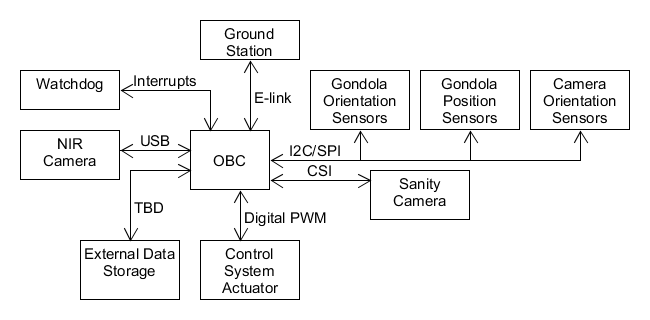
\includegraphics[width=\textwidth]{4-experiment-design/img/software/process-overview.png}
	\caption{Relations between On-Board Computer and connected components.}
	\label{fig:software-process-overview}
\end{figure}

All external components connected to the On-Board Computer and their interface are displayed in figure \ref{fig:software-process-overview}.

\paragraph{b)} General and safety related concepts\\

To ensure that the software is not erroneous rigorous testing will be done during development and after completion. A watchdog timer will be used to avoid software freezing. This timer will reset the On-Board Computer if it is not itself reset by the software within a certain period.

\paragraph{c)} Interfaces\\

If connection to ground is available, images compressed with a lossless compression will be sent down over the E-link over the course of the experiment. If the storage were to fail on touchdown for any reason, this would mean that not all data is lost.


\begin{table}[H]
	\centering
	\begin{tabular}{l|l}
		\textbf{Component}
		& \textbf{Interface} \\ \hline
		Ground Station
		& E-link             \\
		NIR Camera
		& USB                \\
		Guiding Camera
		& USB                \\
		Gondola GPS
		& SPI                \\
		Telescope Gyroscope
		& I2C                \\
		Telescope Encoders
		& I2C                \\
		Controller Actuators
		& I2C                \\
		Thermal Sensors
		& I2C				 \\
		Heaters \& Coolers
		& I2C
	\end{tabular}
	\caption{Table showing the interface that each external component was connected with. This is also visually represented in figure \ref{fig:software-process-overview}.}
	\label{tab:software-interfaces}
\end{table}



\paragraph{d)} Data acquisition and storage\\

The main bulk of data handled is the images taken by the camera. Housekeeping data such as positioning, camera direction, time, etc will also be stored along with the images.

As the camera has a resolution of $5496 * 3672$ and a colour depth of 12\,bits, the raw image size will be 30.27\,MB. For a 4 hour float phase and an exposure time of 30\,s a total of  14.53\,GB is required in on-board data storage for the images.

With a maximum of 1\,Mbit per second data transfer rate to ground it takes at least 145.5\,s to transfer one image compressed losslessly to 60\,\% of original size. This means that with little down time between observations and for most exposure times, not all images can be transmitted to ground.

\paragraph{e)} Process Flow\\

Pre-launch tests shall be conducted to ensure that all systems work as expected. Afterwards the system shall enter a sleep mode with the camera in a safe launch position. When the float phase is reached, the system will wake. After wake-up the system shall find its orientation and the position of the sun. Finally tracking and observation can start.

Astronomical targets are prioritised. The software shall track and observe the highest priority target within the field of view with varying camera settings until one of the following events happen:

\begin{itemize}
	\item Current target leaves operational field of view.
	\item Target moves too close to the sun for observation.
	\item A higher priority target enters the field of view.
\end{itemize}

If one of the aforementioned events happen, the software will switch current target following prioritisation. While observing targets, the On-Board Software shall store images and housekeeping data. If connection to ground is available this data shall be compressed using a lossless compression method and sent to ground.

At the end of the floating phase the camera shall be oriented in a landing position and the system shall shut down. Figure \ref{fig:software-activity-diagram} shows the complete process flow. Figure \ref{fig:software-state-diagram} shows a simple state diagram for the experiment. Observations are done in the Normal state. In the rare case of a software freeze, it will be reset without entering sleep mode. 

\begin{figure}[H]
    \centering
    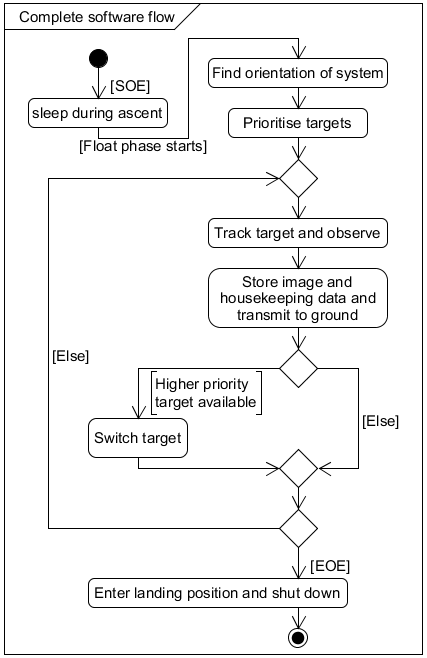
\includegraphics[width=.5\textwidth]{4-experiment-design/img/software/activity-diagram.png}
    \caption{Activity diagram describing the complete software flow.}
    \label{fig:software-activity-diagram}
\end{figure}

\begin{figure}[H]
	\centering
	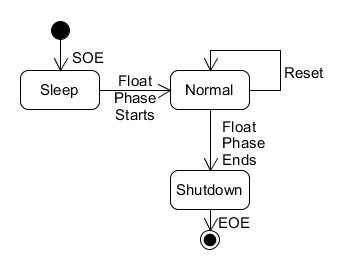
\includegraphics[width=.55\textwidth]{4-experiment-design/img/software/state-diagram.png}
	\caption{State diagram for On-Board Software}
	\label{fig:software-state-diagram}
\end{figure}

\paragraph{f)} Modularisation and pseudo code\\

\begin{figure}[H]
	\centering
	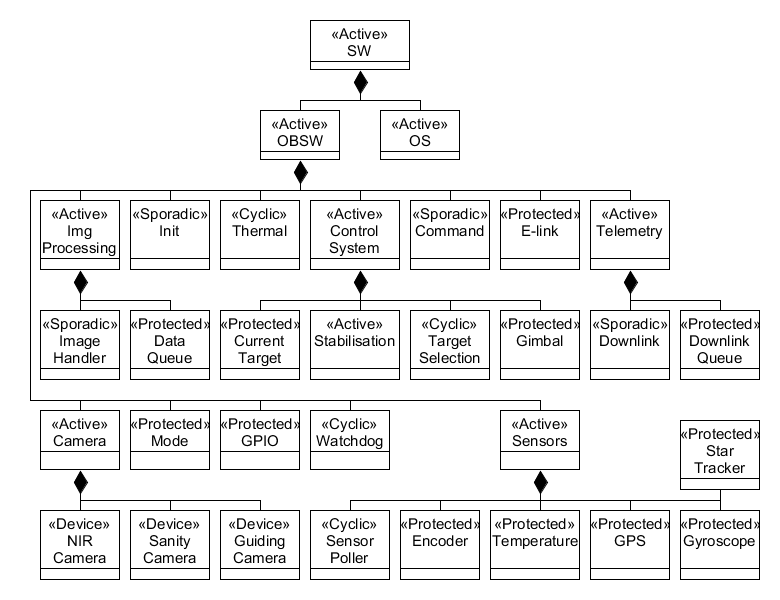
\includegraphics[width=\textwidth]{4-experiment-design/img/software/composition-tree.png}
	\caption{Composition tree of On-Board Software.}
	\label{fig:software-composition-tree}
\end{figure}

Figure \ref{fig:software-composition-tree} shows how the complete software is modularised. Each component is described below.

\begin{itemize}

	\item Img Processing: Image processing, parent
		\begin{itemize}
			\item Image Handler: Module processing and storing images taken by camera.
			\item Data Queue: Buffer to hold camera data until Handler is ready
		\end{itemize}
		
	\item Thermal: Module responsible for active thermal control
	
	\item Watchdog: Timer to reset external watchdog.
	
	\item Tracking: parent
		\begin{itemize}
			\item Current Target: Module holding the current target to be observed.
			\item Controller: Module responsible for keeping camera on target.
			\item Target Choosing: Module responsible for keeping track of target prioritisation.
		\end{itemize}

	\item Init: Module initialising each component.
		
	\item Mode: Module responsible for the current state of the software.
	
	\item Telemetry: Module responsible for sending telemetry to ground.
	
	\item Sensors: parent
		\begin{itemize}
			\item Temperature: Thermal sensors.
			\item Camera Orientation: Module keeping track of camera orientation and location.
			\item Sun: Module keeping track of position of the sun.
		\end{itemize}
		
	\item E-link: Module responsible for communications over the E-link interface. 

	\item I2C: Module responsible for communications over the I2C bus.

	\item SPI: Module responsible for communications over the SPI bus.

	\item Camera: Parent
		\begin{itemize}
			\item Camera Control: Module responsible for selecting target, camera settings and capturing images.
			\item NIR Camera: Communication link to the NIR camera.
			\item Sanity Camera: Communication link to the sanity camera.
			\item Guiding Camera: Communication link to the guiding camera.
		\end{itemize}
		
	\item Command: Module responsible for handling incoming commands from ground.
		
\end{itemize}

\subsubsection{Implementation}

The code for the On-Board Software shall be implemented in C. An operating system will be used to enable the modularisation required. Additional libraries may be needed. 

\subsubsection{Control system}
The main task of the control system is selecting and tracking the astronomical targets and stabilising the telescope during exposure. Other tasks include minor tasks like the thermal control of the CMOS sensor and the electronics box as well as control of the actuators.

\paragraph{Selecting and tracking targets} 

The selection and tracking of targets is done by using the current time, position (GPS) and orientation (compass/magnetometer) of the gondola. Once a suitable target in the operational field of view is selected, it is tracked during exposure. This includes the compensation of the following motions: 
\begin{itemize}
	\item Time-dependent rotational motion of the astronomical targets in the sky. This will be continuously compensated during exposure using models and/or interpolation of tables.
	\item Position-dependent rotational motion of the astronomical targets in the sky. This will be corrected once for every picture, using the GPs data.
	\item Rotation of the gondola in the z-axis; can be corrected during exposure using a gyroscope sensor.
\end{itemize}

Due to the nature of the motion of astronomical targets, it is necessary to use a 3-axis gimbal.

\paragraph{Stabilisation of the gimbal}
The stabilisation of the gimbal only needs to be active during exposure in order to avoid blurred pictures. It is responsible for compensating all kinds of small-scale, unpredicted movements of the gondola. In order to achieve this, an active feedback loop that requires information about the gondola movements is needed. This information is gathered by using accelerometers and gyroscopes for all 3 axis. 


\raggedbottom
